% MBDyn (C) is a multibody analysis code.
% http://www.mbdyn.org
%
% Copyright (C) 1996-2023
%
% Pierangelo Masarati  <pierangelo.masarati@polimi.it>
%
% Dipartimento di Ingegneria Aerospaziale - Politecnico di Milano
% via La Masa, 34 - 20156 Milano, Italy
% http://www.aero.polimi.it
%
% Changing this copyright notice is forbidden.
%
% This program is free software; you can redistribute it and/or modify
% it under the terms of the GNU General Public License as published by
% the Free Software Foundation (version 2 of the License).
%
%
% This program is distributed in the hope that it will be useful,
% but WITHOUT ANY WARRANTY; without even the implied warranty of
% MERCHANTABILITY or FITNESS FOR A PARTICULAR PURPOSE.  See the
% GNU General Public License for more details.
%
% You should have received a copy of the GNU General Public License
% along with this program; if not, write to the Free Software
% Foundation, Inc., 59 Temple Place, Suite 330, Boston, MA  02111-1307  USA

\section{Solid Elements}
\label{sec:EL:SOLID}

\subsection{Displacement based elements}
\emph{Author: Reinhard Resch}

In order to model general three dimensional solid structures subject to large deformations,
large strain and nonlinear material, a generic family of Isoparametric Displacement Based Finite Elements is implemented in MBDyn.
Those elements are based on a Total Lagrangian Formulation according to \cite{BATHE2016}. Shape functions and integration points are based on \cite{BATHE2016}, \cite{DHONDT2004} and \cite{CODEASTERR30301}.
See also table~\ref{sec:EL:SOLID:elemtypes} for a list of supported element types.

\begin{Verbatim}[commandchars=\\\{\}]
    \bnt{elem_type} ::= \{ \kw{hexahedron8} | \kw{hexahedron20} | \kw{hexahedron20r} | \kw{pentahedron15} | \kw{tetrahedron10} \}

    \bnt{normal_arglist} ::=
        [ \kw{static} , ] [ \kw{lumped mass} , ] \bnt{node_data} , \bnt{nodal_density}, \bnt{constitutive_law_data} ;

     \bnt{node_data} :: =
        (\ty{StructDispNode}) \bnt{node_1_label} ,
        (\ty{StructDispNode}) \bnt{node_2_label} ,
        ... ,
        (\ty{StructDispNode}) \bnt{node_N_label}

     \bnt{nodal_density} :: =
        (\ty{real}) \bnt{rho_1}, (\ty{real}) \bnt{rho_2} , ... , (\ty{real}) \bnt{rho_N}

     \bnt{constitutive_law_data} :: =
        \{ \kw{linear elastic isotropic} , \bnt{linear_elastic_isotropic_data} |
           \kw{linear viscoelastic isotropic} , \bnt{linear_viscoelastic_isotropic_data} |
           \bnt{generic_constitutive_law_data} \}


      \bnt{linear_elastic_isotropic_data} :: =
        (\ty{real}) \bnt{E_1} , (\ty{real}) \bnt{nu_1} ,
        \{ (\ty{real}) \bnt{E_2} , (\ty{real}) \bnt{nu_2} | \kw{same} \} ,
        ... ,
        \{ (\ty{real}) \bnt{E_M} , (\ty{real}) \bnt{nu_M} | \kw{same} \}

      \bnt{linear_viscoelastic_isotropic_data} :: =
        (\ty{real}) \bnt{E_1} , (\ty{real}) \bnt{nu_1} , (\ty{real} \bnt{beta_1} ,
        \{ (\ty{real}) \bnt{E_2} , (\ty{real}) \bnt{nu_2} , (\ty{real} \bnt{beta_2} | \kw{same} \} ,
        ... ,
        \{ (\ty{real}) \bnt{E_M} , (\ty{real}) \bnt{nu_M} (\ty{real} \bnt{beta_M} | \kw{same} \}

      \bnt{generic_constitutive_law_data} :: =
        (\htybkw{ConstitutiveLaw}{6D}) \bnt{constitutive_law_1} ,
        \{ (\htybkw{ConstitutiveLaw}{6D}) \bnt{constitutive_law_2} | \kw{same} \} ,
        ... ,
        \{ (\htybkw{ConstitutiveLaw}{6D}) \bnt{constitutive_law_M} | \kw{same} \}
\end{Verbatim}

\subsubsection{Dynamic versus static elements}
By default, dynamic solid elements with inertia effects effects enabled are created,
unless the keyword \kw{static} is used in the element description
or the statement ``\kw{model}: \kw{static}'' was present inside the control data block according section~\ref{sec:CONTROLDATA:MODEL}.
\subsubsection{Gravity and rigid body kinematics}
All solid elements including static ones, are supporting gravity loads according section~\ref{sec:ELEMENTS:gravity}
and rigid body kinematics according section~\ref{sec:CONTROLDATA:RBK}.
\subsubsection{Material properties and constitutive laws}
For that reason, the density of the material must be provided also for static solid elements.
Solid elements may have variable density within a single element.
Also in case of constant density, density values must be provided for each node, and it will be interpolated between nodes.
In addition to linear elastic isotropic and linear viscoelastic isotropic constitutive laws,
any linear or nonlinear elastic or viscoelastic 6D constitutive law can be used if it fulfills the following requirements:
A constitutive law must expect the components of the Green-Lagrange strain tensor $\boldsymbol{G}$
and optionally it's time derivatives $\dot{\boldsymbol{G}}$ as input, and return the components of the Second Piola-Kirchhoff
stress tensor $\boldsymbol{S}$ as output. In addition to generic linear elastic and linear viscoelastic constitutive laws,
also hyperelastic- and elasto-plastic constitutive laws are implemented.
See also section~\ref{sec:CL:neo-hookean}, section~\ref{sec:CL:mooney-rivlin}, section~\ref{sec:CL:bilinear-isotropic-hardening} and section~\ref{sec:CL:linear-viscoelastic-maxwell}.
In case of viscoelastic constitutive laws, the strain rates $\dot{\boldsymbol{\varepsilon}}$ are scaled in order to make
the effect of structural damping independent on the strain \cite{KUEBLER2005}.

\begin{eqnarray}
  \label{sec:EL:SOLID:constlaw}
  \boldsymbol{\sigma} & = & \boldsymbol{f}\left(\boldsymbol{\varepsilon},\, \dot{\boldsymbol{\varepsilon}}^{\star}\right) \\
  \boldsymbol{\sigma} & = & \begin{pmatrix} S_{11} & S_{22} & S_{33} & S_{12} & S_{23} & S_{31} \end{pmatrix}^T \\
  \boldsymbol{\varepsilon} & = & \begin{pmatrix} G_{11} & G_{22} & G_{33} & 2\,G_{12} & 2\,G_{23} & 2\,G_{31} \end{pmatrix}^T \\
  \dot{\boldsymbol{\varepsilon}}^{\star} & = & \begin{pmatrix} \dot{G}_{11}^{\star} & \dot{G}_{22}^{\star} & \dot{G}_{33}^{\star} & 2\,\dot{G}_{12}^{\star} & 2\,\dot{G}_{23}^{\star} & 2\,\dot{G}_{31}^{\star} \end{pmatrix}^T \\
  \dot{\boldsymbol{G}}^{\star} & = & \boldsymbol{C}^{-1} \, \dot{\boldsymbol{G}} \, \boldsymbol{C}^{-1} \, \det{\boldsymbol{F}} \\
  \boldsymbol{G} & = & \frac{1}{2}\,\left(\boldsymbol{C} - \boldsymbol{I}\right) \\
  \boldsymbol{C} & = & \boldsymbol{F}^T\,\boldsymbol{F} \\
  \boldsymbol{F} & = & \nabla \boldsymbol{u} + \boldsymbol{I}
\end{eqnarray}
\begin{description}
\item[$\boldsymbol{f}$] Constitutive law
\item[$\boldsymbol{G}$] Green-Lagrange strain tensor
\item[$\boldsymbol{S}$] Second Piola-Kirchhoff stress tensor
\item[$\boldsymbol{C}$] Right Cauchy-Green strain tensor
\item[$\boldsymbol{F}$] Deformation gradient
\item[$\boldsymbol{u}$] Deformation field
\end{description}
One constitutive law must be provided per integration point.
As a consequence it is possible to build elements with varying elastic properties across a single element.
The actual number of integration points is shown in table~\ref{sec:EL:SOLID:elemtypes}.
\subsubsection{Output}
\paragraph{Output of stress and strain}
By default six components of the Cauchy stress tensor $\bar{\boldsymbol{\tau}}$ and six strains $\bar{\boldsymbol{\varepsilon}}$ at element nodes are written to the output file.
See also equation~\ref{SEC:EL:solid:output:start} to equation~\ref{SEC:EL:solid:output:end} which are based on \cite{WALLRAPP1998}.
Since stress and strain are evaluated at integration points instead of nodes, it is required to extrapolate $\bar{\boldsymbol{\tau}}$ and $\bar{\boldsymbol{\varepsilon}}$
from integration points to nodes using Lapack's DGELSD function.
\begin{eqnarray}
  \boldsymbol{\tau} & = & \frac{1}{\det{\boldsymbol{F}}} \, \boldsymbol{F} \, \boldsymbol{S} \, \boldsymbol{F}^T   \label{SEC:EL:solid:output:start} \\
  \bar{\varepsilon}_{\alpha} & = & \sqrt{C_{\alpha\alpha}} - 1 \\
  \sin{\vartheta_{\alpha\beta}} & = & \frac{C_{\alpha\beta}}{\left(1 + \bar{\varepsilon}_{\alpha}\right)\left(1 + \bar{\varepsilon}_{\beta}\right)}   \label{SEC:EL:solid:output:end}  \\
  \bar{\boldsymbol{\tau}} & = & \begin{pmatrix}
    \tau_{11} &
    \tau_{22} &
    \tau_{33} &
    \tau_{12} &
    \tau_{23} &
    \tau_{31}
  \end{pmatrix}^T \\
  \bar{\boldsymbol{\varepsilon}} & = & \begin{pmatrix}
    \bar{\varepsilon}_1 &
    \bar{\varepsilon}_2 &
    \bar{\varepsilon}_3 &
    \sin{\vartheta}_{12} &
    \sin{\vartheta}_{23} &
    \sin{\vartheta}_{31}
  \end{pmatrix}^T
\end{eqnarray}

\paragraph{Output of accelerations}
By default dynamic solid elements are using a consistent mass matrix. In order to enable output of accelerations
for dynamic structural nodes, it is required to use a lumped mass matrix.
For that purpose the keyword \kw{lumped mass} must be used.
Due to the special handling of accelerations in MBDyn, only solid elements with lumped mass matrix enabled
can be used to compute accelerations for structural nodes as described in section~\ref{sec:NODE:STRUCTURAL:SYNTAX:accel}.

\begin{table}[h!tp]
\begin{tabular}[t]{|c|c|c|c|c|c|c|}
  \hline
  element type & nodes & node order & integration points & order & integration & references \tabularnewline
  \hline
  \kw{hexahedron8} & 8 & \ref{fig:EL:SOLID:HEXAHEDRON8} & 8 & 1 & full & \cite{BATHE2016} \tabularnewline
  \hline
  \kw{hexahedron20} & 20 & \ref{fig:EL:SOLID:HEXAHEDRON20} & 27 & 2 & full & \cite{BATHE2016} \tabularnewline
  \hline
  \kw{hexahedron20r} & 20 & \ref{fig:EL:SOLID:HEXAHEDRON20R} & 8 & 2 & reduced & \cite{DHONDT2004} \tabularnewline
  \hline
  \kw{pentahedron15} & 15 & \ref{fig:EL:SOLID:PENTAHEDRON15} & 21 & 2 & full & \cite{CODEASTERR30301} \tabularnewline
  \hline
  \kw{tetrahedron10} & 10 & \ref{fig:EL:SOLID:TETRAHEDRON10H} & 5 & 2 & full & \cite{CODEASTERR30301} \tabularnewline
  \hline
\end{tabular}
\caption{Finite Element Types for solid elements}
\label{sec:EL:SOLID:elemtypes}
\end{table}


\paragraph{Private Data}
\label{sec:EL:SOLID:PRIVATE}
The following private data is available:
\begin{enumerate}
\item \kw{"E"} Kinetic energy
\end{enumerate}
Kinetic energy is always zero if the keyword \kw{static} was used.

\begin{figure}[htb]
\centering 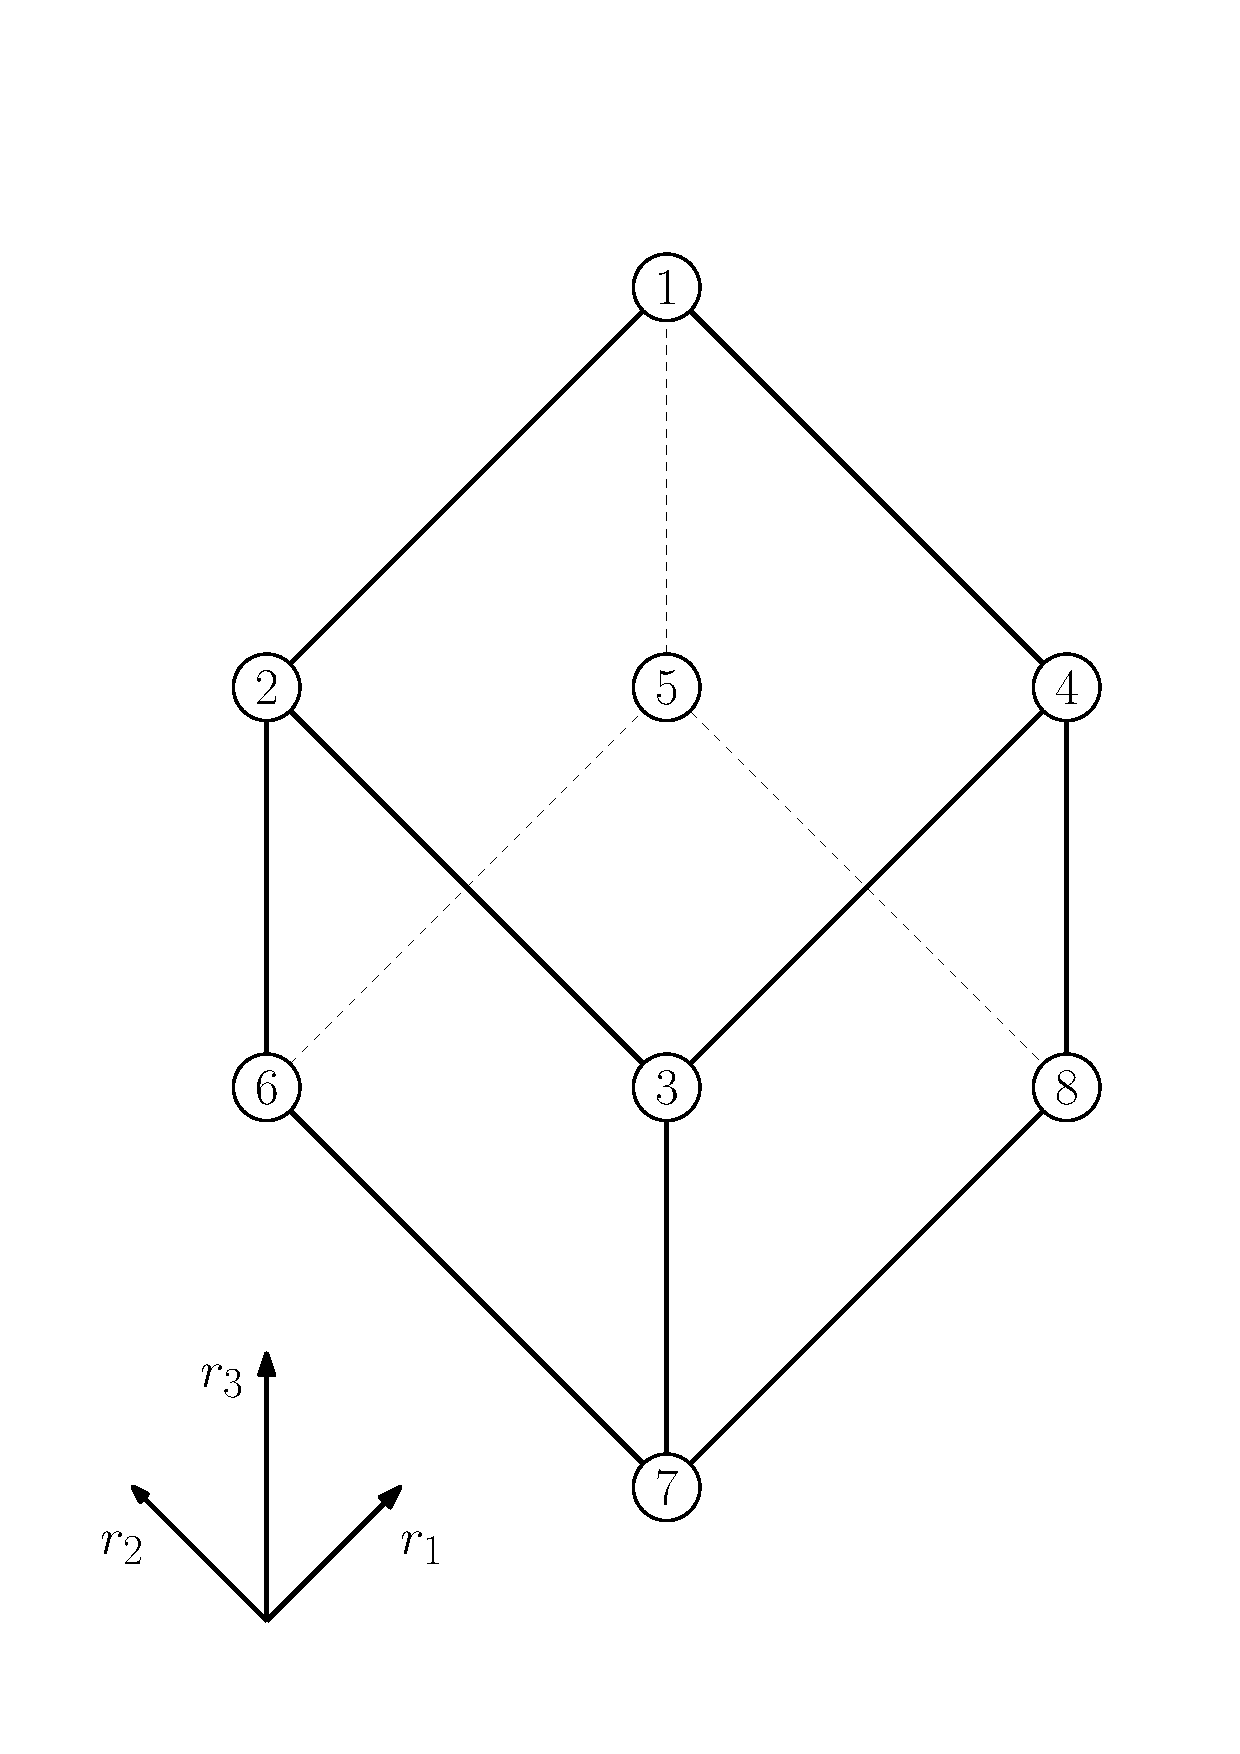
\includegraphics[width=.25\textwidth]{hexahedron8}
\caption{Node order: hexahedron8}
\label{fig:EL:SOLID:HEXAHEDRON8}
\end{figure}

\begin{figure}[htb]
\centering
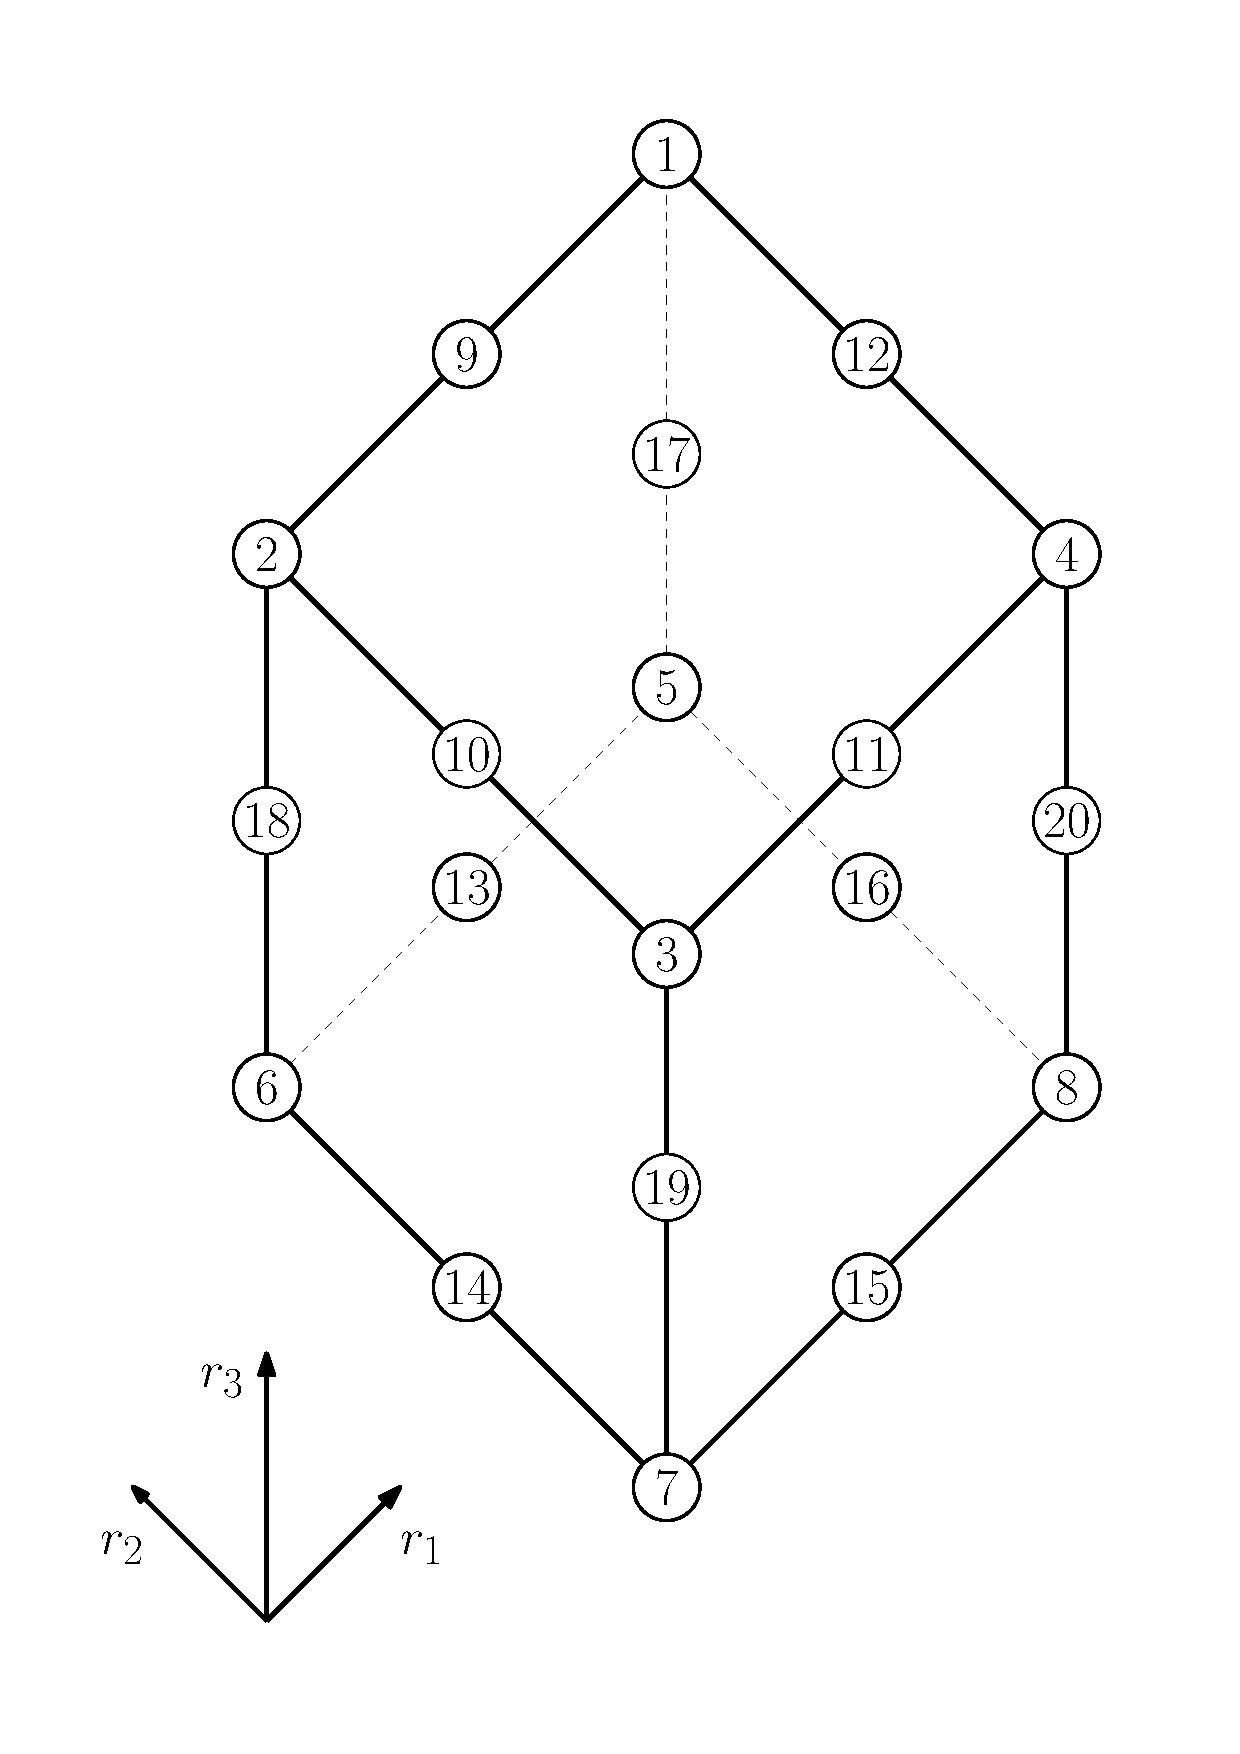
\includegraphics[width=.25\textwidth]{hexahedron20}
\caption{Node order: hexahedron20}
\label{fig:EL:SOLID:HEXAHEDRON20}
\end{figure}

\begin{figure}[htb]
\centering
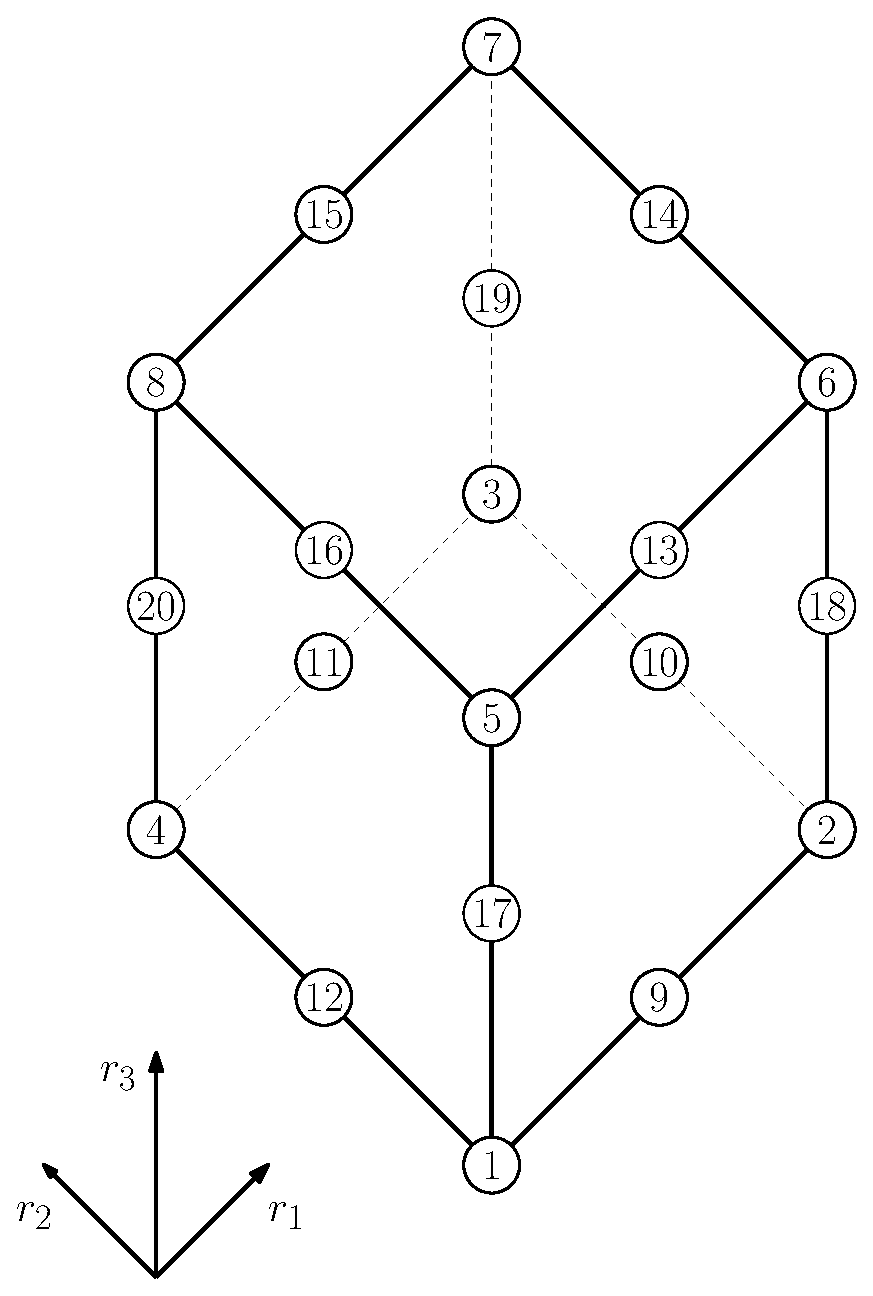
\includegraphics[width=.25\textwidth]{hexahedron20r}
\caption{Node order: hexahedron20r}
\label{fig:EL:SOLID:HEXAHEDRON20R}
\end{figure}

\begin{figure}[htb]
\centering
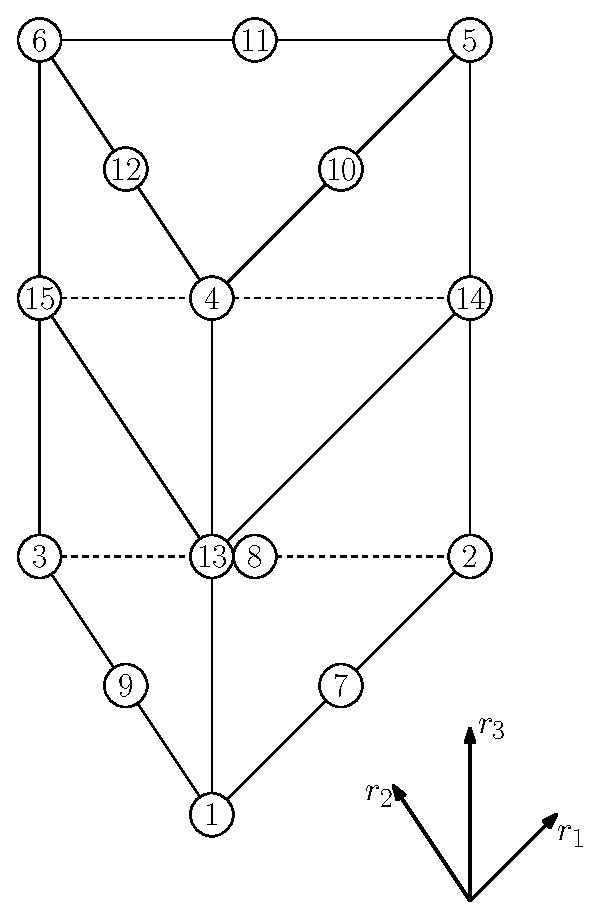
\includegraphics[width=.25\textwidth]{pentahedron15}
\caption{Node order: pentahedron15}
\label{fig:EL:SOLID:PENTAHEDRON15}
\end{figure}

\begin{figure}[htb]
\centering
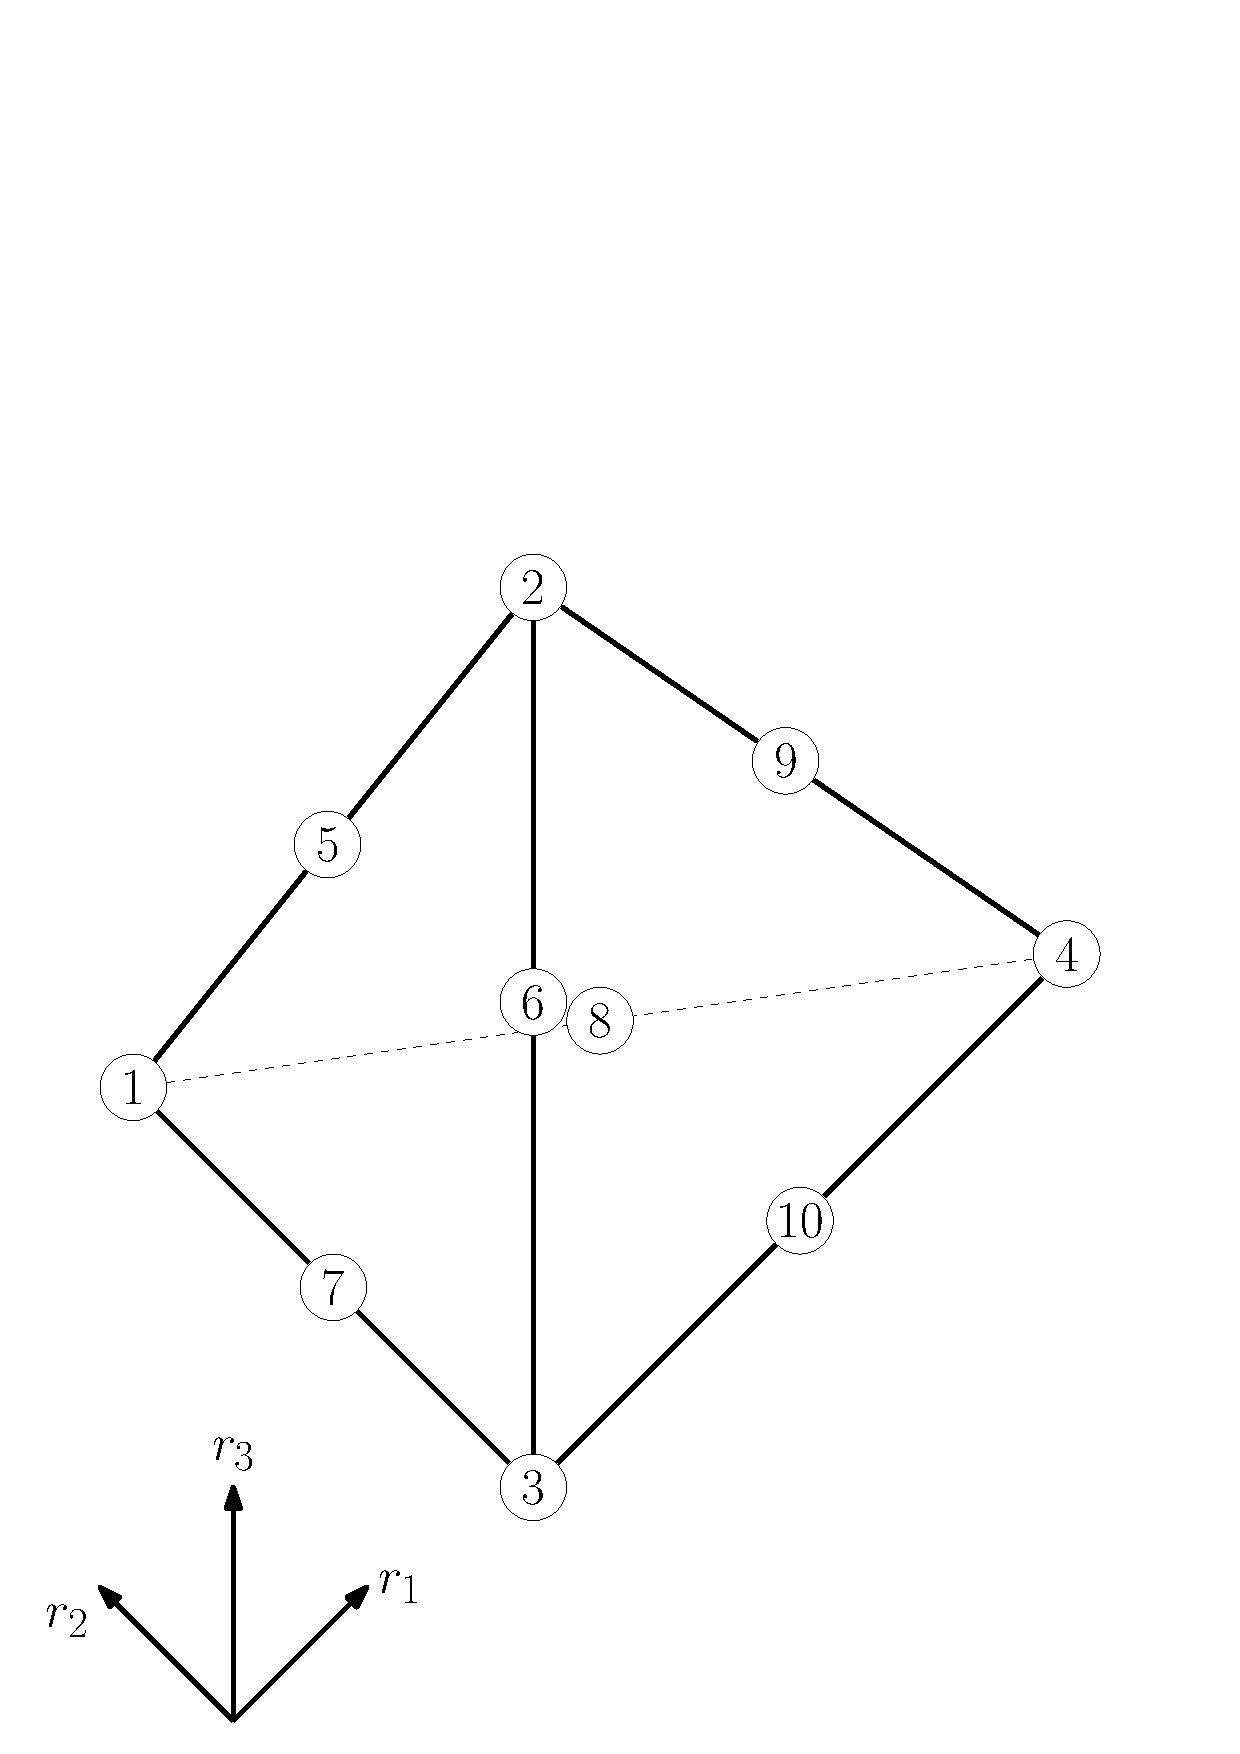
\includegraphics[width=.25\textwidth]{tetrahedron10h}
\caption{Node order: tetrahedron10}
\label{fig:EL:SOLID:TETRAHEDRON10H}
\end{figure}

\subsubsection{Example:}
\begin{verbatim}
    constitutive law: 1, name, "solid1", 6,
             linear viscoelastic generic,
             matr , 2.82e+11, 1.21e+11, 1.21e+11, 0.00e+00, 0.00e+00, 0.00e+00,
                    1.21e+11, 2.82e+11, 1.21e+11, 0.00e+00, 0.00e+00, 0.00e+00,
                    1.21e+11, 1.21e+11, 2.82e+11, 0.00e+00, 0.00e+00, 0.00e+00,
                    0.00e+00, 0.00e+00, 0.00e+00, 8.07e+10, 0.00e+00, 0.00e+00,
                    0.00e+00, 0.00e+00, 0.00e+00, 0.00e+00, 8.07e+10, 0.00e+00,
                    0.00e+00, 0.00e+00, 0.00e+00, 0.00e+00, 0.00e+00, 8.07e+10,
                    proportional, 1.0e-04;

    hexahedron8: 100, 1, 2, 3, 4, 5, 6, 7, 8,
                  7850., 7850., 7850., 7850., 7850., 7850., 7850., 7850.,
                  reference, 1, same, same, same, same, same, same, same;

    hexahedron8: 101, 5, 6, 7, 8, 9, 10, 11, 12,
                  7850., 7850., 7850., 7850., 7850., 7850., 7850., 7850.,
                  linear elastic isotropic, 210000e6, 0.3, same, same, same, same, same, same, same;
\end{verbatim}

\subsubsection{Pre- and post-processing}
\label{sec:EL:SOLID:preprocessing}
Since it would become tedious to create the mesh manually, pre- and post-processing of solid models
can be performed by means of \htmladdnormallink{\texttt{GNU Octave}}{https://octave.org/},
\htmladdnormallink{\texttt{mboct-fem-pkg}}{https://github.com/octave-user/mboct-fem-pkg}
and \htmladdnormallink{\texttt{Gmsh}}{https://gmsh.info/}.
See also the following example and figure~\ref{fig:EL:SOLID:COOKS-MEMBRANE} on how to generate the input files and how to load the output generated by MBDyn:

\begin{Verbatim}[commandchars=\\\{\}]
  \ty{## load the package}
  pkg load mboct-fem-pkg;
  \ty{## load the mesh file in Gmsh format}
  mesh = \nt{fem_pre_mesh_import}(\kw{"cooks_membrane.msh"}, \kw{"gmsh"});
  \ty{## Apply a fill in reducing ordering based on METIS}
  mesh = \nt{fem_pre_mesh_reorder}(mesh);
  \ty{## assign material properties to material number 1}
  mesh.material_data(\kw{1}).E = \kw{240000}; \ty{## Young's modulus [Pa]}
  mesh.material_data(\kw{1}).nu = \kw{0.49}; \ty{## Poisson's ratio [1]}
  mesh.material_data(\kw{1}).rho = \kw{1000}; \ty{## density [kg/m^3]}
  mesh.material_data(\kw{1}).type = \kw{"neo hookean"}; \ty{## hyperelastic rubber like material}
  \ty{## allocate material assignment}
  mesh.materials.iso20 = \nt{zeros}(\nt{rows}(mesh.elements.iso20), 1, \kw{"int32"});
  \ty{## locate a group of solid elements with id 10}
  grp_idx_solid = \nt{find}([[mesh.groups.iso20].id] == \kw{10});
  \ty{## locate a group of surface elements with id 12}
  grp_idx_clamp = \nt{find}([[mesh.groups.quad8].id] == \kw{12});
  \ty{## assign the material number one to all elements in group 10}
  mesh.materials.iso20(mesh.groups.iso20(grp_idx_solid).elements) = \kw{1};
  \ty{## allocate a new node number}
  node_id_interface = \nt{rows}(mesh.nodes) + \kw{1};
  \ty{## define the position of a new node}
  mesh.nodes(node_id_interface, \kw{1}:\kw{3}) = [\kw{100e-3}, \kw{50e-3}, \kw{20e-3}];
  \ty{## create an RBE3 element for the interface node (this will become a rigid body displacement joint)}
  \ty{## all nodes inside group 13 will be coupled to the interface node}
  mesh.elements.rbe3 = \nt{fem_pre_mesh_rbe3_from_surf}(mesh, \kw{13}, node_id_interface, \kw{"quad8"});
  \ty{## allocate the DOF status for all nodes}
  load_case_dof.locked_dof = \nt{false}(\nt{size}(mesh.nodes));
  \ty{## lock all DOF's at surface number 12}
  load_case_dof.locked_dof(mesh.groups.quad8(grp_idx_clamp).nodes, \kw{1}:\kw{3}) = \nt{true};
  \ty{## apply a force Fx = 5N * sin(2 * pi * t) and Fy = 5N * cos(2 * pi * t) at the interface node}
  load_case(\kw{1}).loads = [\kw{5}, \kw{0}, \kw{0}, \kw{0}, \kw{0}, \kw{0}];
  load_case(\kw{2}).loads = [\kw{0}, \kw{5}, \kw{0}, \kw{0}, \kw{0}, \kw{0}];
  load_case(\kw{1}).loaded_nodes = [node_id_interface];
  load_case(\kw{2}).loaed_nodes = [node_id_interface];
  opts.forces.time_function = \{\kw{'string, "sin(2 * pi * Time)"'}, \kw{'string, "cos(2 * pi * Time)"'}\};
  \ty{## define the node type for all displacement only nodes with three degrees of freedom}
  opts.struct_nodes.type = \nt{repmat}(\nt{MBDYN_NODE_TYPE_DYNAMIC_STRUCT_DISP}, \nt{rows}(mesh.nodes), \kw{1});
  \ty{## make sure that a static structural node}
  \ty{## with six degrees of freedom is created for the interface node}
  opts.struct_nodes.type(node_id_interface) = \nt{MBDYN_NODE_TYPE_STATIC_STRUCT};
  \ty{## write all the nodes to file "cooks_membrane.nod"}
  opts = \nt{mbdyn_pre_solid_write_nodes}(mesh, \kw{"cooks_membrane.nod"}, opts);
  \ty{## write all the constitutive laws to file "cooks_membrane.csl"}
  opts = \nt{mbdyn_pre_solid_write_const_laws}(mesh, \kw{"cooks_membrane.csl"}, opts);
  \ty{## write all the elements to file "cooks_membrane.elm"}
  opts = \nt{mbdyn_pre_solid_write_elements}(mesh, load_case_dof, load_case, \kw{"cooks_membrane.elm"}, opts);
  \ty{## define the location of the output file}
  opt_sol.output_file = \kw{"cooks_membrane_output"};
  \ty{## run MBDyn}
  info = \nt{mbdyn_solver_run}(\kw{"cooks_membrane.mbd"}, opt_sol);
  \ty{## load the output}
  [mesh_sol, sol] = \nt{mbdyn_post_load_output_sol}(opt_sol.output_file);
  \ty{## display results using Gmsh}
  \nt{fem_post_sol_external}(mesh_sol, sol);
\end{Verbatim}

\begin{figure}[htb]
\centering
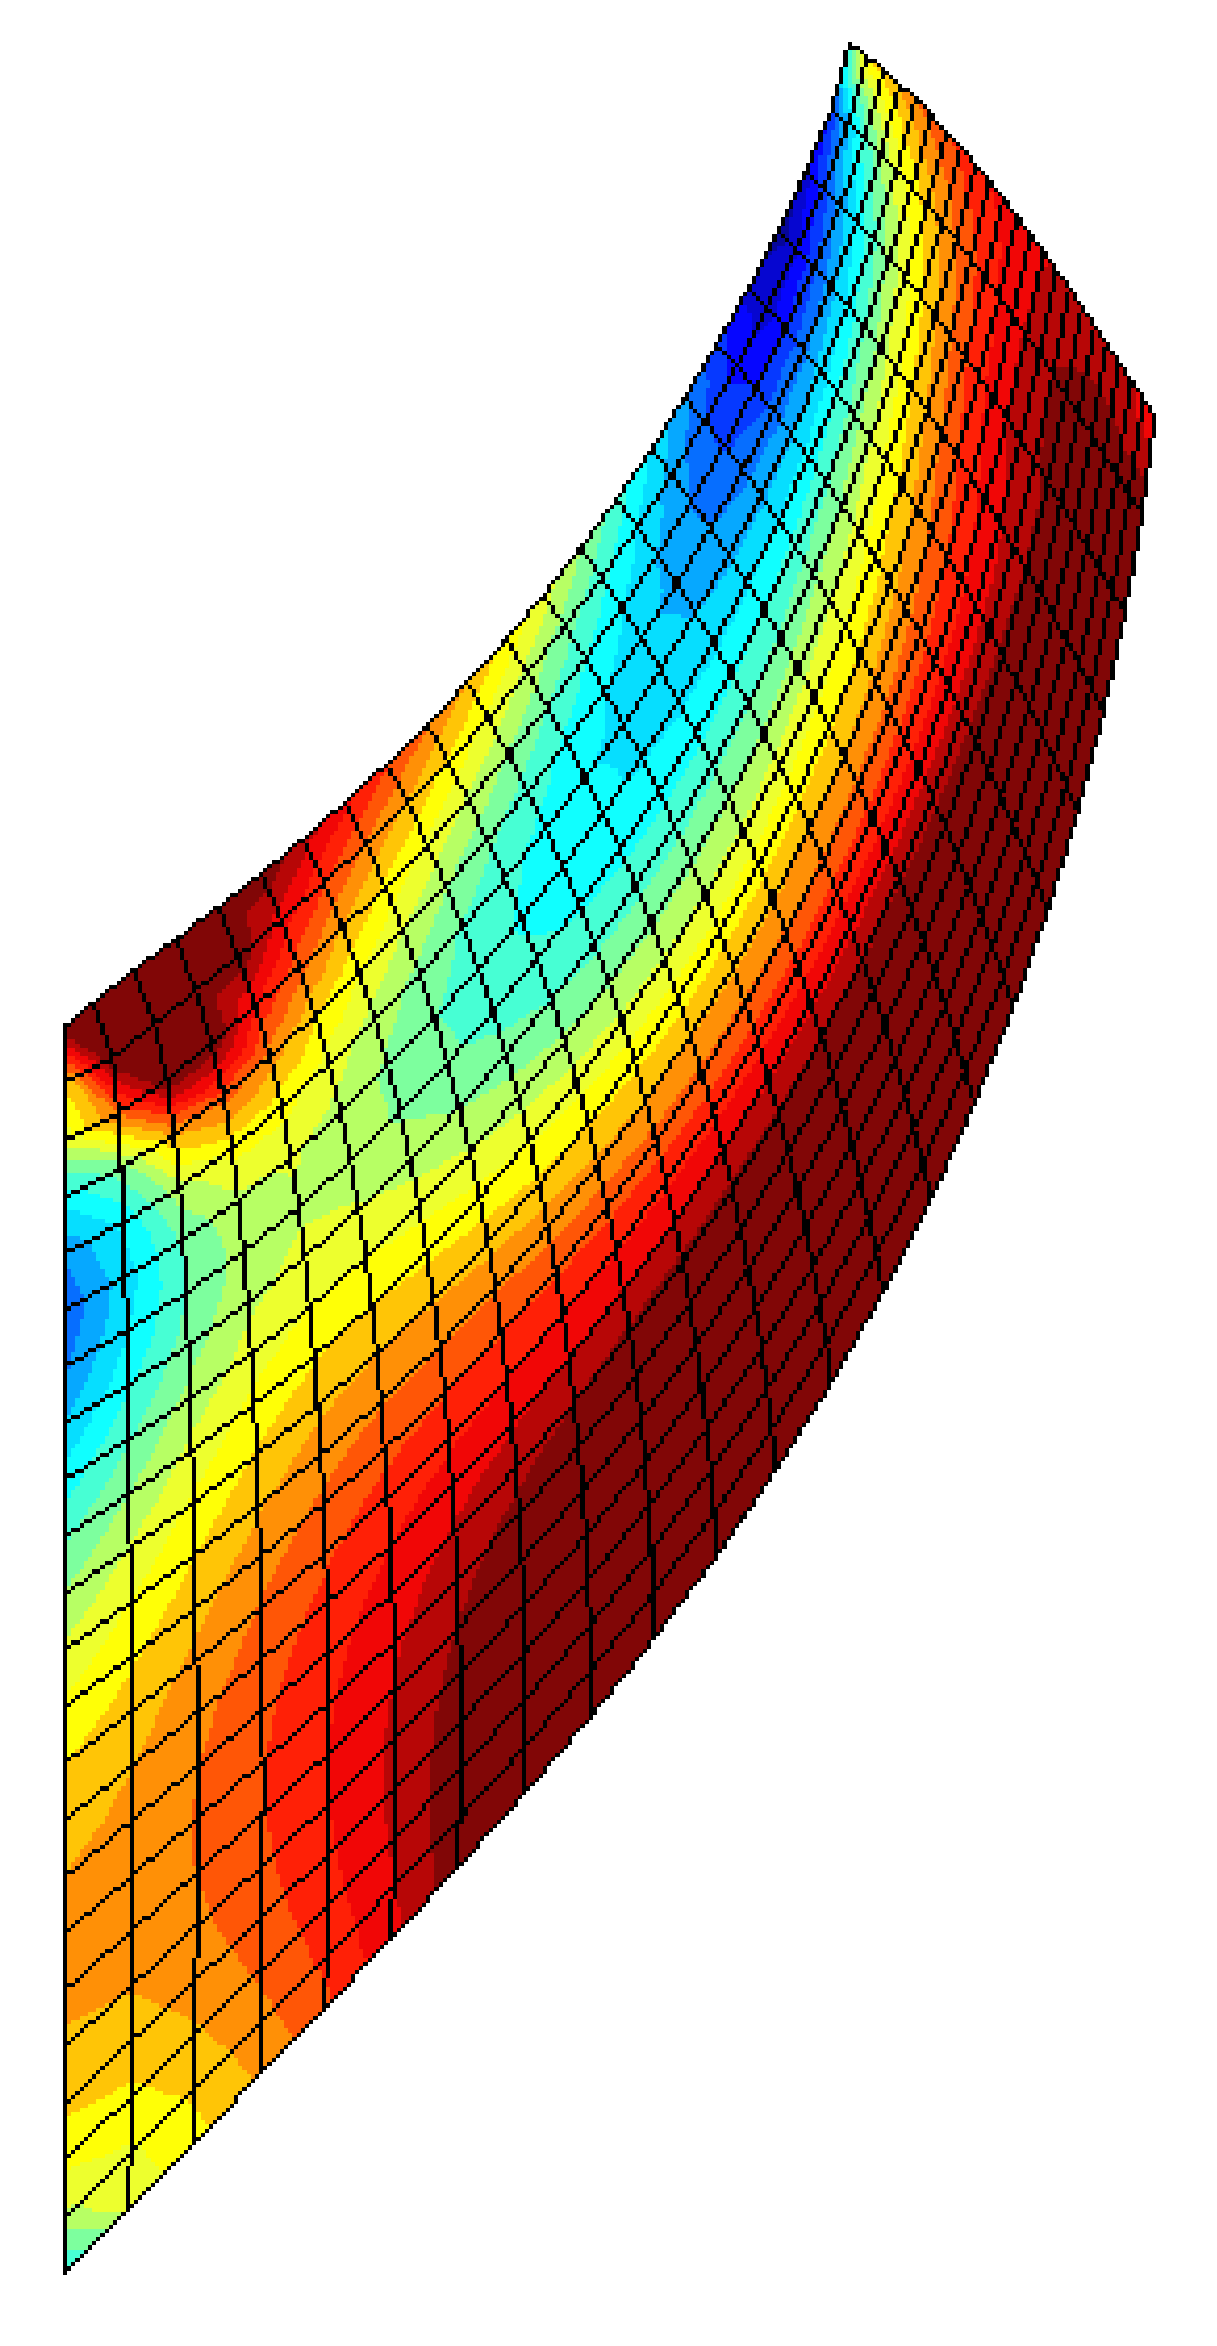
\includegraphics[width=.25\textwidth]{elemsolid}
\caption{Cook's membrane: deformed shape and Von Mises stress rendered using Gmsh}
\label{fig:EL:SOLID:COOKS-MEMBRANE}
\end{figure}
\clearpage
